\documentclass[tikz,border=4pt]{standalone}
\usepackage[utf8]{inputenc}
\usepackage[T1]{fontenc}
\usetikzlibrary{positioning,arrows.meta,shapes.multipart}
\definecolor{gcn}{HTML}{2a78d6}
\definecolor{base}{HTML}{eb6834}
\definecolor{tinta}{HTML}{52514e}
\begin{document}
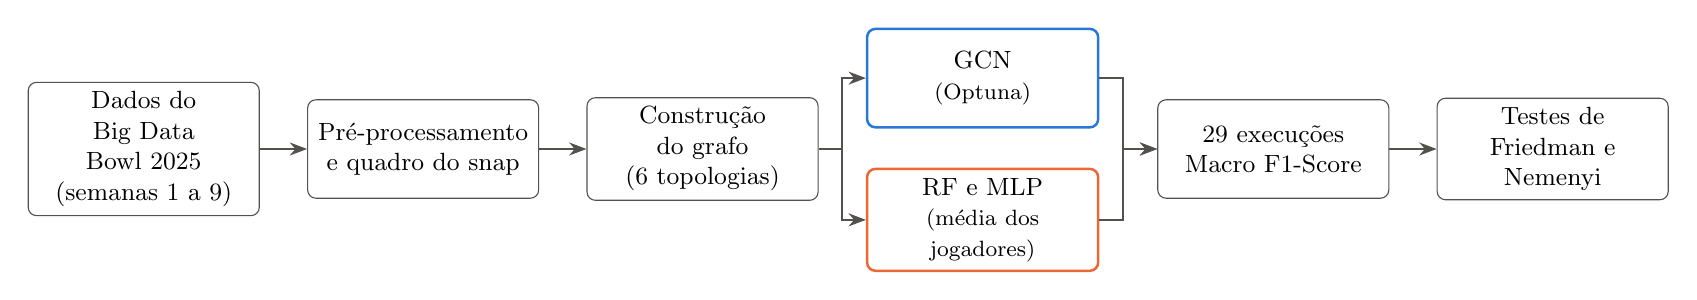
\begin{tikzpicture}[
  font=\small,
  caixa/.style={draw=tinta, rounded corners=3pt, align=center, minimum height=1.25cm, text width=2.7cm, fill=white},
  seta/.style={-{Stealth[length=2.2mm]}, thick, draw=tinta},
  node distance=0.55cm and 0.6cm]
\node[caixa] (dados) {Dados do\\Big Data Bowl 2025\\(semanas 1 a 9)};
\node[caixa, right=of dados] (pre) {Pr\'e-processamento\\e quadro do snap};
\node[caixa, right=of pre] (grafo) {Constru\c{c}\~ao do grafo\\(6 topologias)};
\node[caixa, right=of grafo, yshift=0.9cm, draw=gcn, line width=0.9pt] (gcn) {GCN\\{\footnotesize (Optuna)}};
\node[caixa, right=of grafo, yshift=-0.9cm, draw=base, line width=0.9pt] (bl) {RF e MLP\\{\footnotesize (m\'edia dos jogadores)}};
\node[caixa, right=1.0cm of grafo, xshift=3.3cm] (aval) {29 execu\c{c}\~oes\\Macro F1-Score};
\node[caixa, right=of aval] (est) {Testes de\\Friedman e\\Nemenyi};
\draw[seta] (dados) -- (pre);
\draw[seta] (pre) -- (grafo);
\draw[seta] (grafo.east) -- ++(0.3,0) |- (gcn.west);
\draw[seta] (grafo.east) -- ++(0.3,0) |- (bl.west);
\draw[seta] (gcn.east) -- ++(0.3,0) |- (aval.west);
\draw[seta] (bl.east) -- ++(0.3,0) |- (aval.west);
\draw[seta] (aval) -- (est);
\end{tikzpicture}
\end{document}
